\documentclass{standalone}

\usepackage{lscape}
%Math typesetting packages
\usepackage{amsfonts, amssymb, amsmath, latexsym, amsthm,xparse, bm}
\newcommand\simiid{\stackrel{iid}{\sim}}
\newcommand\simind{\stackrel{ind}{\sim}}
\NewDocumentCommand{\qfrac}{smm}{%
  \dfrac{\IfBooleanT{#1}{\vphantom{\big|}}#2}{\mathstrut #3}%
}

\usepackage{tikz}
\usetikzlibrary{calc,arrows,positioning,shapes,shapes.gates.logic.US,trees, intersections}

\begin{document}

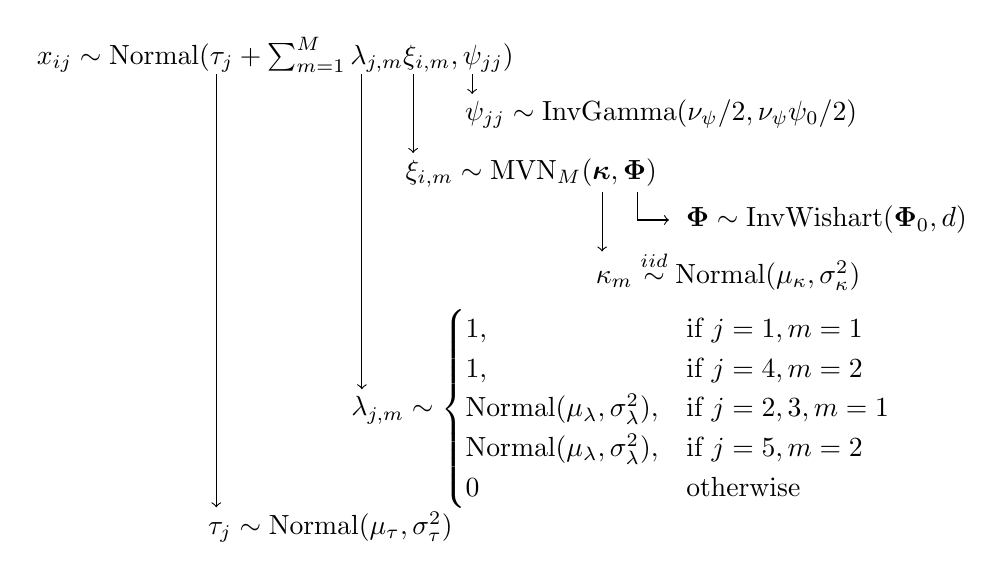
\begin{tikzpicture}
  \node at (0,0) {$x_{ij} \sim \mathrm{Normal}(\tau_j + \sum_{m=1}^M\lambda_{j,m}\xi_{i,m}, \psi_{jj})$} ;
  	\draw[->] (2.5, -0.25) -- (2.5, -0.5);
  	\node at (4.9, -0.75) {$\psi_{jj}\sim \mathrm{InvGamma}(\nu_{\psi}/2, \nu_{\psi}\psi_0/2)$};
  		%\draw[->] (6, -1) |- (6.3, -1.25);
  		%\node at (7, -1.25) {$\psi_0 = 2$};
  		%\draw[->] (4.6, -1) -- (4.6, -1.25);
  		%\node at (5.15, -1.5) {$\nu_{\psi} = 10$};
  	\draw[->] (1.75,-0.25) -- (1.75,-1.25);
  	\node at (3.25, -1.5) {$\xi_{i,m} \sim \mathrm{MVN}_{M}(\bm\kappa,\bm\Phi)$};
  		\draw[->] (4.6, -1.75) |- (5, -2.1);
  		\node at (7, -2.1) {$\bm\Phi\sim \mathrm{InvWishart}(\bm\Phi_0, d)$};
  		\draw[->] (4.15, -1.75) -- (4.15, -2.5);
	  	\node at (5.75, -2.75) {$\kappa_m \simiid \mathrm{Normal}(\mu_{\kappa},\sigma^2_{\kappa})$};
	  	
	\draw[->] (1.1,-0.25) -- (1.1,-4.25);
  	\node at (4.40, -4.5) {$\lambda_{j,m} \sim \begin{cases} 1, & \text{if}\ j=1, m=1\\ 1, & \text{if}\ j=4, m=2\\ \mathrm{Normal}(\mu_{\lambda}, \sigma^2_{\lambda}),&  \text{if}\ j=2,3, m=1 \\ \mathrm{Normal}(\mu_{\lambda}, \sigma^2_{\lambda}),& \text{if}\ j=5, m=2 \\ 0 & \text{otherwise} \end{cases}$};
  	\draw[->] (-0.75, -0.25) -- (-0.75, -5.75);
  	\node at (0.7, -6) {$\tau_j \sim \mathrm{Normal}(\mu_{\tau},\sigma^2_{\tau})$};
  		
\end{tikzpicture}

\end{document}